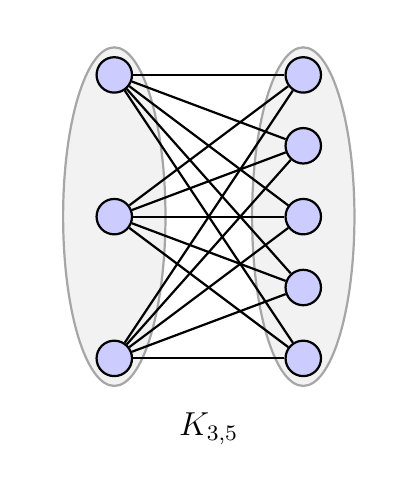
\begin{tikzpicture}[
  baseline=0pt,
  scale=1,
  vnode/.style={circle, draw=black, fill=blue!20, thick, inner sep=0pt, minimum size=4.5mm},
  edge/.style={thick, draw=black}
]
  \useasboundingbox (-2.3,-3.1) rectangle (2.3,2.4);

  % Conjuntos de la partición (Venn)
  \draw[thick, draw=gray!70, fill=gray!10] (-1.2, 0) ellipse [x radius=0.65cm, y radius=2.15cm];
  \draw[thick, draw=gray!70, fill=gray!10] (1.2, 0) ellipse [x radius=0.65cm, y radius=2.15cm];

  % Vértices Partición Izquierda (3 vértices)
  \node[vnode] (a1) at (-1.2, 1.8) {};
  \node[vnode] (a2) at (-1.2, 0.0) {};
  \node[vnode] (a3) at (-1.2, -1.8) {};

  % Vértices Partición Derecha (5 vértices)
  \node[vnode] (b1) at (1.2, 1.8) {};
  \node[vnode] (b2) at (1.2, 0.9) {};
  \node[vnode] (b3) at (1.2, 0.0) {};
  \node[vnode] (b4) at (1.2, -0.9) {};
  \node[vnode] (b5) at (1.2, -1.8) {};

  % Aristas (Todas las conexiones)
  \foreach \i in {1,2,3} {
    \foreach \j in {1,...,5} {
      \draw[edge] (a\i) -- (b\j);
    }
  }

  % Etiqueta inferior
  \node[font=\large] at (0,-2.7) {$K_{3,5}$};
\end{tikzpicture}
